\chapter{Návrhové vzory Flux a Redux}

\label{kap:vzory} % id kapitoly pre prikaz ref

V tejto kapitole si povieme niečo o návrhových vzoroch Flux a Redux, ktoré sú určené na spracovávanie udalostí v aplikácii.

\section{Flux}
Hlavné črty návrhového vzoru Flux. \cite[Overview]{Flux}

Flux je vzor pre spravovanie dát v aplikácii. Najdôležitejším konceptom je tok informácií jedným smerom. Obsahuje štyri základné časti. \emph{Akcie}, ktoré vytvára používateľ, prostredie, kde aplikácia beží alebo aj časti aplikácie. \emph{Dispečer} spravuje všetky vytvorené akcie. \emph{Store}, ktorý reaguje na akcie a mení data aplikácie a \emph{View}, ktorý data aplikácie vykresľuje.
%TODO odkaz na obrazok

%TODO zdroj
% zdroj: https://facebook.github.io/flux/img/flux-simple-f8-diagram-with-client-action-1300w.png

\begin{figure}
  \centering
    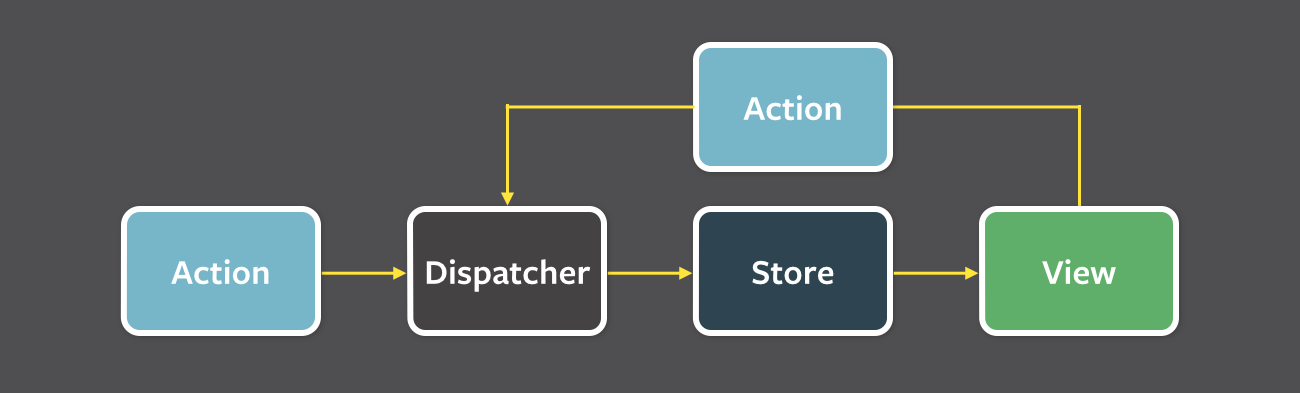
\includegraphics[width=\textwidth]{./images/flux.png}
  \caption{Flux architektúra}
\end{figure}

\subsection{Dispečer}
Dispečer spravuje všetky akcie vykonané v aplikácii. V celej aplikácii by mal byť len jeden. Dispečer obsahuje callback %TODO preložiť
na každý Store v aplikácii. Keď sa vykoná nová akcia, dispečer pošle túto akciu všetkým Storom. Sám nemusí obsahovať akúkoľvek vyššiu logiku, slúži len na distribúciu.

\subsection{Store}
Story obsahujú stav a logiku aplikácie. Store reaguje na akciu, na základe ktorej môže zmeniť data, ktoré spravuje. Storov môže byť viac a každý upravuje nejakú podčasť dát. Každý store poskytuje Dispečerovi callback na seba, aby keď sa udeje nejaká akcia, bol o tom upozornený. Na základe typu akcie sa rozhodne, či a ako bude meniť data aplikácie. (Napríklad ak máme dva story Images a Texts, tak pri vytvorení akcie EditText sa pravdepodobne store Image rozhodne nič nerobiť.) Po zmene dát vytvorí udalosť, ktorou upozorní View časť, že treba prekresliť údaje.

\subsection{Akcie}
Akcie definujú internú API aplikácie. Zachytávajú možnosti interakcie s aplikáciou. Sú to jednoduché objekty s kľúčom \emph{typ} a voliteľnými pridanými informáciami. Typ akcie by nemal obsahovať žiadne implementačné detaily.

Akcie vytvára View časť ( napríklad keď reagujeme na stlačenie tlačidla ), %TODO medzery okolo zátvoriek
server (napríklad chybová hláška počas komunikácie) %TODO
alebo aj store (keď odstránime používateľa, chceme odstrániť aj všetky jeho príspevky).

\begin{lstlisting}[caption=Akcia vo Flux architektúre]
  {
  	type: 'delete-user',
  	userId: '1'
  }
\end{lstlisting}

\subsection{Views}%TODO ako písať data vs dáta
View časť je tá, ktorá vykresľuje dáta zo storu. Aby bola táto časť vždy aktuálna, musí daný view komponent počúvať na všetky udalosti od storu, ktoré hovoria o zmene relevantných dát. Ak sa zmenia dáta, store vytvorí udalosť a view sa prekreslí. Architektúra flux neurčuje, ako majú byť tieto data vykreslené.






\section{Redux}
Hlavné črty návrhového vzoru Redux. 

Redux je popis spracovania udalostí v aplikácii. Dáva do popredia lieárne spracovanie udalosti. Pozostáva z troch hlavných častí, jeden \emph{store}, v ktorom sú všetky dáta aplikácie uložené, \emph{reducer} - čistú funkciu, ktorá jediná mení akokoľvek stav aplikácie a komponenty, ktoré dané data zo stavu vykresľujú.

%TODO obrázok

\subsection{Store}
Store, správca stavu, vystupuje ako jediný zdroj pravdy v aplikácii. Všetky data, ktoré sú vykreslené, pochádzajú zo stavu. Teda ak poznáme tento stav, veľmi jednoducho vieme potom nasimulovať prostredie, v ktorom celá aplikácia beží. Rovnako v prípade chýb vieme oveľa jednoduchšie zistiť, kde chyba nastala. Tento stav je nemenný(immutable). Ak ho chceme teda zmeniť, musíme vytvoriť novú inštanciu, v ktorej urobíme potrebné zmeny. Toto je dôležité, aby sme vedeli sledovať beh aplikácie.
%dispatch

Store má svoju funkciu \emph{dispatch()} ktorá slúži na prijímanie podnetov zvonka, aby store zmenil svoj stav.

\subsection{Komponenty}% TODO rozdiel medzi užívateľ a používateľ?
Komponenty slúžia na vykreslenie stavu aplikácie pre užívateľa. Ponúkajú rozhranie pre používateľa na komunikáciu s programom a v prípade reduxovej aplikácie je to práve pomocou vytvárania akcií. Komponenty vieme rozdeliť na "múdre" a "hlúpe".%TODO pojmy! :D
Hlúpe komponenty iba vykresľujú data, ktoré dostanú. Tieto sú potom veľmi ľahko znovupoužiteľné. Tie múdre komunikujú spätne s dátami. V reduxovej aplikácii poskytujú rozhranie pre vytváranie akcií a majú prístup ku funkcii dispatch.

\subsection{Akcie}
Akcia je akákoľvek udalosť, ktorá sa môže v aplikácii vyskytnúť, od stlačenia tlačidla užívateľom, až po chybové hlášky alebo stiahnutie dát zo servera. Na vytvorenie akcie používame funkciu dispatch. Každá akcia musí obsahovať typ a môže voliteľne obsahovať aj nejaké prídavné data. Na základe tejto akcie potom reducer vypočíta nový stav.

\subsection{Reducer}% TODO side effects!
Všetká logika aplikácie sa deje v reduceroch. Reducery sú jediný objekt, ktorý môže meniť stav aplikácie.

Reducer je čistá funkcia. Má dva argumenty, stav aplikácie a akciu, ktorá sa vykonala a výstupom je nový stav. Vďaka tejto vlastnosti, že nemá žiadne "side effects" ju môžeme veľmi ľahko testovať.

Reducer môžeme vyskladať z viacerých menších čistých funkcií, kde každá z nich sa stará len o určitú malú časť stavu. Vďaka tomu zostáva kód prehľadný a jednoduchý.% nejaḱe kecy o funkcionalnom programovani?
Pri písaní reduceru nesmieme zabúdať na to, že nový stav, ktorý vrátime, nesmie byť "starý prerobený" ale musíme ho prekopírovať a dáta zmeniť až v novej inštancii.

\subsection{Middlewares}
Niekedy treba robiť aj akcie, ktoré nevieme robiť lineárne, nemôžeme robiť lineárne, alebo na ne len nechceme čakať. Príkladom je dopyt na server, kedy čas príchodu odpovede nezávisí úplne od nášho programu. Vtedy môžeme použiť...%TODO







\section{Knižnice open source}%TODO preložiť?

\paragraph{Este}
Celú aplikáciu sme začali vyvýjať v prostredí este. Snaha držať sa agilného prístupu vývoja aplikácie nás nasmerovala na využitie čo najviac už existujúceho kódu. %Táto zbierka knižníc ...

 \cite[Este starter kit]{Este}

\paragraph{React}
Na vykreslenie komponentov sme pri vývoji použili knižnicu React. Jej veľkou výhodou je, že je rozšírená medzi programátormi a existuje pre ňu mnoho ďalších kompatibilných knižníc. Tiež veľmi pekne spolupracuje s našim návrhovým vzorom \emph{Redux}, keďže React-ové komponenty majú úlohu iba dáta vykresliť.

\paragraph{Komponenty material dizajnu}

react-toolbox

material-ui
- onTouchTap
- vhodné pre natívne aplikácie a pre mobilné aplikácie
- my vyvíjame aplikáciu pre prehliadač

\paragraph{Router}%TODO preložiť?
O niečo zložitejšie je routovanie a správa url v aplikácii. Existuje viacero možností, ako riešiť routovanie. 

Na túto funkciu sme využili knižnicu react-router. Jej výhodou je, že routovanie z komponentov je veľmi jednoduché a prirodzené. Čo mne osobne chýbalo, bola málo popísaná možnosť meniť adresu mimo komponentov. Túto vlastnosť by sme veľmi ocenili najmä kôli ideológii Redux-u, keďže tu by mal byť jediným zdojom pravdy práve stav aplikácie v stave. Po použití tejto knižnice máme "zdroje pravdy" aspoň dva, jeden pre dáta aplikácie a druhý pre adresu url. %Podarilo sa mi tento nedostatok odstrániť funkciou push do histórie prehliadača.
%TODO uvodzovky

Trošku "krajšie" v zmysle redux-ovej logiky by bolo riešenie s použitím knižnice router-5, ktorá rieši celý routing na základe dát v stave, kam si aj ukladá informácie o aktuálnej adrese (aj predchádzajúcich).% TODO uvodzovky

\cite[gettting started]{Redux}






\section{Porovnanie vzorov Flux a Redux}
Popis spracovania udalostí v oboch vzoroch a ich vzájomné porovnanie. Vymenovanie a zhrnutie spoločných znakov a rozdielnych.

\section{Postrehy}
V reduxe je funkcia reducer čistá funkcia. Preto vždy pri písaní funkcií sme sa sústredili na písanie takýchto funkcií, ktoré sa neskôr lepšie skladajú. Heslo jedna funkcia má robiť jednu vec sme preferovali pre lepšiu prehľadnosť a čitateľnosť kódu.

Pri mixinoch sme si spomínali, že tieto objekty sme premenili na čisté funkcie. Toto nám veľmi vyhovuje v prípade reduxového návrhu.

\section{Návrhy migrácie Flux do Redux}%alebo len porovnanie?
Viaceré možné návrhy migrácie s referenciami na existujúce návrhy na internete.

\section{Riešenie}
Jedno vybrané riešenie z vyššie uvedených. Zdôvodnenie a návrh implementácie mnou zvoleného riešenia.

